\documentclass{sigchi}

% pandoc setup %



\usepackage[backend=biber]{biblatex}
\addbibresource{references.bib}

\providecommand{\tightlist}{%
  \setlength{\itemsep}{0pt}\setlength{\parskip}{0pt}}

% end pandoc setup %

% Use this section to set the ACM copyright statement (e.g. for
% preprints).  Consult the conference website for the camera-ready
% copyright statement.

% Copyright
\CopyrightYear{2020}
%\setcopyright{acmcopyright}
\setcopyright{acmlicensed}
%\setcopyright{rightsretained}
%\setcopyright{usgov}
%\setcopyright{usgovmixed}
%\setcopyright{cagov}
%\setcopyright{cagovmixed}
% DOI
\doi{https://doi.org/10.1145/3313831.XXXXXXX}
% ISBN
\isbn{978-1-4503-6708-0/20/04}
%Conference
\conferenceinfo{CHI'20,}{April  25--30, 2020, Honolulu, HI, USA}
%Price
\acmPrice{\$15.00}

% Use this command to override the default ACM copyright statement
% (e.g. for preprints).  Consult the conference website for the
% camera-ready copyright statement.

%% HOW TO OVERRIDE THE DEFAULT COPYRIGHT STRIP --
%% Please note you need to make sure the copy for your specific
%% license is used here!
% \toappear{
% Permission to make digital or hard copies of all or part of this work
% for personal or classroom use is granted without fee provided that
% copies are not made or distributed for profit or commercial advantage
% and that copies bear this notice and the full citation on the first
% page. Copyrights for components of this work owned by others than ACM
% must be honored. Abstracting with credit is permitted. To copy
% otherwise, or republish, to post on servers or to redistribute to
% lists, requires prior specific permission and/or a fee. Request
% permissions from \href{mailto:Permissions@acm.org}{Permissions@acm.org}. \\
% \emph{CHI '16},  May 07--12, 2016, San Jose, CA, USA \\
% ACM xxx-x-xxxx-xxxx-x/xx/xx\ldots \$15.00 \\
% DOI: \url{http://dx.doi.org/xx.xxxx/xxxxxxx.xxxxxxx}
% }

% Arabic page numbers for submission.  Remove this line to eliminate
% page numbers for the camera ready copy
% \pagenumbering{arabic}

% Load basic packages
\usepackage{balance}       % to better equalize the last page
\usepackage{graphics}      % for EPS, load graphicx instead
\usepackage[T1]{fontenc}   % for umlauts and other diaeresis
\usepackage{txfonts}
\usepackage{mathptmx}
\usepackage[pdflang={en-US},pdftex]{hyperref}
\usepackage{color}
\usepackage{booktabs}
\usepackage{textcomp}

% Some optional stuff you might like/need.
\usepackage{microtype}        % Improved Tracking and Kerning
% \usepackage[all]{hypcap}    % Fixes bug in hyperref caption linking
\usepackage{ccicons}          % Cite your images correctly!
% \usepackage[utf8]{inputenc} % for a UTF8 editor only

% If you want to use todo notes, marginpars etc. during creation of
% your draft document, you have to enable the "chi_draft" option for
% the document class. To do this, change the very first line to:
% "\documentclass[chi_draft]{sigchi}". You can then place todo notes
% by using the "\todo{...}"  command. Make sure to disable the draft
% option again before submitting your final document.
\usepackage{todonotes}

% Paper metadata (use plain text, for PDF inclusion and later
% re-using, if desired).  Use \emtpyauthor when submitting for review
% so you remain anonymous.
\def\plaintitle{Abstract Program Visualization for Model-View-Update
User Interfaces}
\def\plainauthor{Geoffrey Litt}
\def\emptyauthor{}
\def\plainkeywords{Program visualization, program understanding, debugging}
\def\plaingeneralterms{Program visualization, program understanding, debugging}

% llt: Define a global style for URLs, rather that the default one
\makeatletter
\def\url@leostyle{%
  \@ifundefined{selectfont}{
    \def\UrlFont{\sf}
  }{
    \def\UrlFont{\small\bf\ttfamily}
  }}
\makeatother
\urlstyle{leo}

% To make various LaTeX processors do the right thing with page size.
\def\pprw{8.5in}
\def\pprh{11in}
\special{papersize=\pprw,\pprh}
\setlength{\paperwidth}{\pprw}
\setlength{\paperheight}{\pprh}
\setlength{\pdfpagewidth}{\pprw}
\setlength{\pdfpageheight}{\pprh}

% Make sure hyperref comes last of your loaded packages, to give it a
% fighting chance of not being over-written, since its job is to
% redefine many LaTeX commands.
\definecolor{linkColor}{RGB}{6,125,233}
\hypersetup{%
  pdftitle={\plaintitle},
% Use \plainauthor for final version.
%  pdfauthor={\plainauthor},
  pdfauthor={\plainauthor},
  pdfkeywords={\plainkeywords},
  pdfdisplaydoctitle=true, % For Accessibility
  bookmarksnumbered,
  pdfstartview={FitH},
  colorlinks,
  citecolor=black,
  filecolor=black,
  linkcolor=black,
  urlcolor=linkColor,
  breaklinks=true,
  hypertexnames=false
}

% create a shortcut to typeset table headings
% \newcommand\tabhead[1]{\small\textbf{#1}}

% End of preamble. Here it comes the document.
\begin{document}

\title{\plaintitle}

\numberofauthors{1}
\author{%
  \alignauthor{Geoffrey Litt}\\
    \affaddr{MIT CSAIL}\\
    \email{glitt@mit.edu}\\
}

\maketitle

\begin{abstract}
  Visualizing the runtime behavior of programs can help programmers with
  targeted debugging and general understanding. For understanding
  complex programs, visualizations abstracted from the low-level code
  are most helpful, but this introduces new challenges: how does the
  programmer specify what to visualize, and how do we visualize complex
  data structures which aren't just primitive values? In this work, I
  present an approach to visualizing the behavior of user interfaces
  built with the Model-View-Update pattern. I present a prototype
  runtime visualization system built on the Redux library and argue
  that, by exploiting the natural abstraction characteristics of this
  application architecture, we can create useful runtime visualizations
  with minimal programmer effort.
\end{abstract}


% ACM Classfication

\begin{CCSXML}
<ccs2012>
<concept>
<concept_id>10003120.10003121</concept_id>
<concept_desc>Human-centered computing~Human computer interaction (HCI)</concept_desc>
<concept_significance>500</concept_significance>
</concept>
<concept>
<concept_id>10003120.10003121.10003125.10011752</concept_id>
<concept_desc>Human-centered computing~Haptic devices</concept_desc>
<concept_significance>300</concept_significance>
</concept>
<concept>
<concept_id>10003120.10003121.10003122.10003334</concept_id>
<concept_desc>Human-centered computing~User studies</concept_desc>
<concept_significance>100</concept_significance>
</concept>
</ccs2012>
\end{CCSXML}

\ccsdesc[500]{Human-centered computing~Human computer interaction (HCI)}
\ccsdesc[300]{Human-centered computing~Haptic devices}
\ccsdesc[100]{Human-centered computing~User studies}

% Author Keywords
\keywords{\plainkeywords}

% Print the classficiation codes
% \printccsdesc
% Please use the 2012 Classifiers and see this link to embed them in the text: \url{https://dl.acm.org/ccs/ccs_flat.cfm}

\hypertarget{introduction}{%
\section{Introduction}\label{introduction}}

Much recent work in program visualization
\autocite{victora,guo2013,hoffswell2018a,pollock2019,kasibatla2018}
focuses on low-level details: showing the values of individual
variables, connected to individual lines of source code. This makes
sense for small programs, and for helping novices understand the basics
of programming languages. But these visualizations don't address the
needs of more experienced programmers working with larger programs.
Gaining a general understanding of a large program requires zooming out
far above the source code level.

This leads to the idea of \emph{abstract program visualization}:
creating abstract, program-specific views of runtime state or static
code, to help someone understand the program. This idea has been
explored in the context of teaching how algorithms work
\autocite{brown1984,stasko1990} and in understanding the behavior of
multithreaded Java programs \autocite{reiss2003,reiss2005}. In this
context, a tricky challenge emerges \autocite{reiss2007}: how can we
simultaneously tailor the visualization to the specific domain, while
enabling the programmer to create the visualization with minimal effort?
On the one hand, overly generic visualizations (as used in low-level
visualization systems like Python Tutor \autocite{guo2013}) will often
fail to capture the higher-level context of the specific program. On the
other hand, if a visualization is too specific and takes too much work
to create, it won't be reasonably possible for programmers to create the
visualization.

I think a promising strategy for approaching this problem is to create
runtime visualization systems coupled to a particular domain-specific
framework or language. Frameworks and DSLs often impose a particular
mental model, code architecture style, and other constraints that
usefully narrow the space of possible programs relative to a
general-purpose language. On the other hand, there are still many
different programs that can be built in one framework, so the effort of
building a visualization system can be amortized over thousands of
programs rather than concentrated on a single one.

One recent example of this strategy is visualizing runtime state in Vega
\autocite{hoffswell2018a}, a data visualization language. Because the
language is so domain-specific, the runtime visualization system is able
to make many contextual assumptions leading to a useful visualization.

In this work, I propose a runtime program visualization system for a
slightly more general category of applications: user interfaces built
with the Model-View-Update (MVU) architecture \autocite{fowler2020},
also commonly known as the Elm Architecture \autocite{czaplicki}. MVU
encourages the state of the interface to be centralized in a single data
structure, derived by running a pure reducer function over a stream of
events.

This architecture has been found to have many practical benefits for
program understanding and developer experience (e.g., making
``time-travel debugging'' relatively trivial to implement), but I think
it also has useful characteristics for abstract program visualization as
well. In particular, MVU naturally encourages programmers to define
abstractions that represent the essence of their application: 1) a
stream of semantically meaningful events, representing important changes
in the application, 2) a state object that represents all the core state
of the UI, organized in a hierarchical way. My hypothesis is that it's
possible to build a system that can visualize MVU interfaces with
relatively little additional effort from the programmer, because of
these natural characteristics of the architecture.

To begin to explore this idea, I've prototyped a runtime visualization
system on top of the popular Redux \autocite{zotero-621} Javascript
library. Within the limited scope of this project, I've focused
specifically on making a prototype specifically designed to visualize
the state of the TodoMVC demo application. I've designed some
visualization formats tailored to the state of that application, and
through my own usage I've begun to gain a preliminary understanding what
kinds of visualizations might be useful to programmers navigating the
state of MVU applications over time.

Much future work remains to fully flesh out this idea, including:

\begin{itemize}
\tightlist
\item
  developing a crisper understanding of the needs of programmers who are
  debugging MVU applications or trying to gain a general understanding
  of their behavior
\item
  generalizing the system so that it actually works with many Redux
  applications instead of just one, and has a way for a programmer to
  create a program-specific visualization
\end{itemize}

\hypertarget{sec:related-work}{%
\section{Related Work}\label{sec:related-work}}

Reiss \autocite{reiss2007} provides a useful taxonomy of execution
visualizations, with pointers to prior research. Some particularly
relevant dimensions for this work include abstract vs concrete, and
effort required to create the visualization.

Many systems have explored visualizing execution state at the level of
individual source lines, including Learnable Programming
\autocite{victora}, Python Tutor \autocite{guo2013}, Omnicode
\autocite{kang2017}, Theia \autocite{pollock2019}, and Theseus
\autocite{lieber2014}.

Some systems have explored somewhat more abstract views. Projection
Boxes {[}\textcite{lerner2020} provides a way of selectively showing
parts of application state, and Seymour \autocite{kasibatla2018}
provides a ``macro'' visualization to generally show the layout of
execution flow, in addition to a ``micro'' visualization.

Other systems have explored fully abstract program visualization,
entirely disconnected from the source code. For example, Balsa
\autocite{brown1984} and Tango \autocite{stasko1990} show animated views
of algorithms operating, and Jive \autocite{reiss2003} and Jove
\autocite{reiss2005} visualize various high-level projections of the
execution of Java programs, e.g.~when different threads are running.

Hoffswell et al propose a system for visualizing runtime state inside
Vega data visualizations \autocite{hoffswell2018a}. That work fits into
the category of visualizing state next to source code lines, but by
integrating with a very high level domain-specific language, achieves
more abstraction than visualization systems for general languages like
Python. They also propose a design space for visualizations embedded in
source code, which I plan to build on in this work.

\hypertarget{sec:design}{%
\section{Visualization design}\label{sec:design}}

\hypertarget{use-cases}{%
\subsection{Use cases}\label{use-cases}}

I had some prior experience with the Redux Dev Tools system, which
provides the ability to inspect application state in Redux applications.
From this personal experience I identified two distinct use cases for a
runtime visualization:

\begin{itemize}
\tightlist
\item
  \textbf{Localizing within a trace}: \emph{Where do I need to rewind
  to, in order to inspect a particularly relevant point in an execution
  trace?} This is most often helpful when debugging a particular
  problem. Scrubbing back and forth while watching the UI change is a
  manageable solution, but it's inefficient, and sometimes the relevant
  state isn't directly visible in the UI.
\item
  \textbf{Generally understanding program behavior over time}:
  \emph{Overall, what happened as I interacted with the program?}
  Sometimes I'm not debugging a particular problem, and I'm more
  interested in just seeing general information about how a program is
  behaving over time. This is helpful when explaining the system's
  behavior to a new programmer who's preparing to work on the system, or
  for building up my own passive understanding of a system.
\end{itemize}

These two goals partially overlap, but can also lead in different design
directions. For example, localizing a specific point in a trace can
benefit from a more active interrogatory approach (e.g.~as explored in
the Whyline system \autocite{ko2004}), but general program understanding
might benefit from a more passive interaction style.

\hypertarget{data-structures}{%
\subsection{Data structures}\label{data-structures}}

Many concrete and low-level program visualizations focus on showing
primitive values, especially numeric values. However, the state of an
arbitrary MVU application often contains complex nested data structures,
which contain many non-numeric values: booleans, strings, and enum
values. One challenge for this system is to find ways to visualize these
types of structures.

\hypertarget{sec:design}{%
\section{Visualization Design}\label{sec:design}}

\hypertarget{context-todomvc}{%
\subsection{Context: TodoMVC}\label{context-todomvc}}

In order to focus my effort on concretely understanding the utility of
visualizations, rather than building out infrastructure, I built a
visualization system for a specific application: the Redux
implementation of the TodoMVC GUI benchmark. TodoMVC is a basic todo
list UI where you can add, edit, delete, and complete todos. You can
filter the list of todos shown to either active or completed ones.

In Redux, the implementation stores an app state object as shown in
Figure~\ref{fig:todomvc-state}. There are Redux actions corresponding to
each of the main actions listed above, e.g.~``add todo'' and ``set
visibility filter''. Importantly, the Redux events capture an abstract,
semantically meaningful picture of the user's interactions: when adding
a new todo, the user's keystrokes are collected in the local state of a
React component, and only a single ``add todo'' event is triggered in
Redux once the user finally adds the new todo.

\begin{figure}
\hypertarget{fig:todomvc-state}{%
\centering
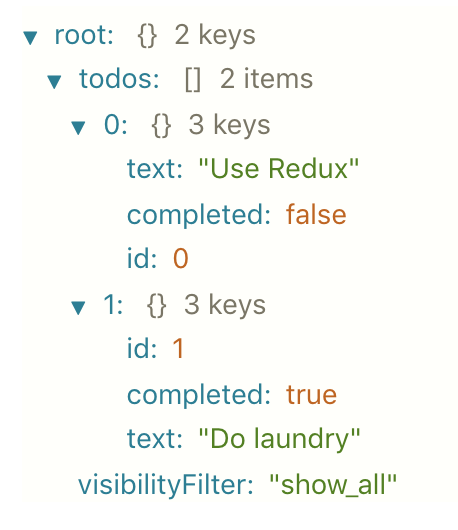
\includegraphics[width=1.82292in,height=2.08333in]{images/todomvc-state.png}
\caption{TodoMVC Redux application state}\label{fig:todomvc-state}
}
\end{figure}

\hypertarget{overall-layout}{%
\subsection{Overall layout}\label{overall-layout}}

\begin{figure}
\hypertarget{fig:mockup}{%
\centering
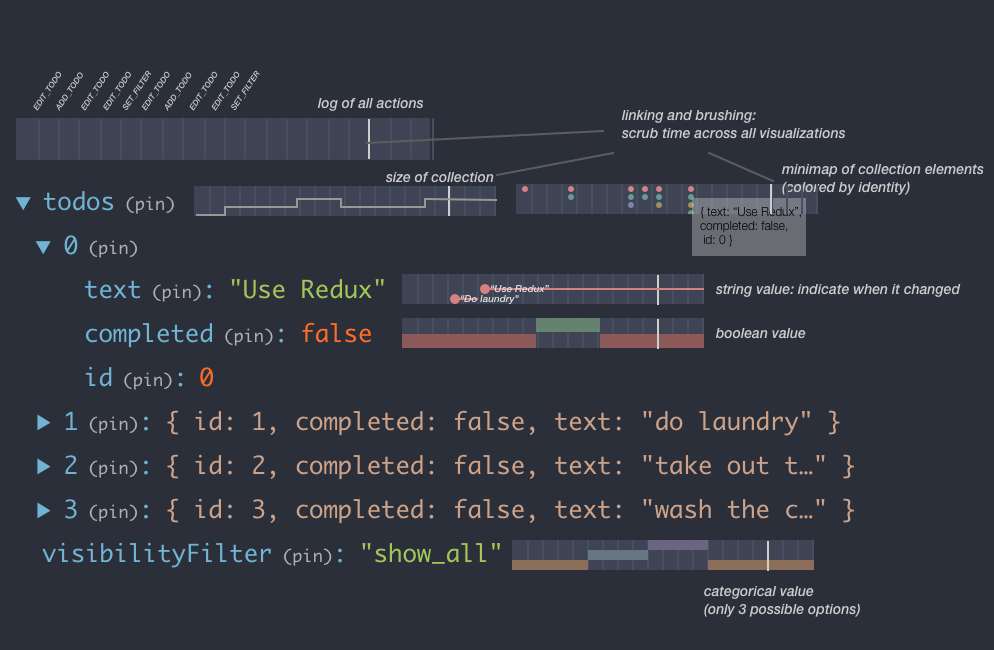
\includegraphics[width=3.4375in,height=2.25in]{images/mockup.png}
\caption{JSON tree with inline sparklines}\label{fig:mockup}
}
\end{figure}

My initial idea, as shown in Figure~\ref{fig:mockup}, was to show the
current state of the application as a nested JSON tree, and then to show
small sparkline-style visualizations next to nodes of the tree. This
design draws some inspiration from \autocite{hoffswell2018a}, but
differs in that it uses visualization to annotate the application's
state tree, rather than its source code. The advantage of this design is
that it closely and directly links the current state to data from the
execution history, but that link also causes thorny problems---for
example, how do you deal with nodes that have disappeared from the
current state? Perhaps more concerningly, by tying the visualization to
the \emph{concrete} current state, it limits the ability of the
programmer to create a customized abstract view. Linking the
visualization to the Redux state is a much more abstract view than
linking to lines of source code, but it still presents a limitation.

As a result, in my next iteration I switched to a different layout,
shown in Figure~\ref{fig:timeline}: a vertically stacked list of small
visualizations of state over time. Each visualization can display an
arbitrary projection of the app's Redux state. Because the graphs are
horizontally aligned, it's easy to see how different aspects of the
app's state have changed in relation to each other. While I haven't
implemented this yet, I imagine that programmers would be able to
dynamically add visualizations to this list, specifying useful
projections of app state, and deciding what type of visualization to use
for each projection.

\begin{figure}
\hypertarget{fig:timeline}{%
\centering
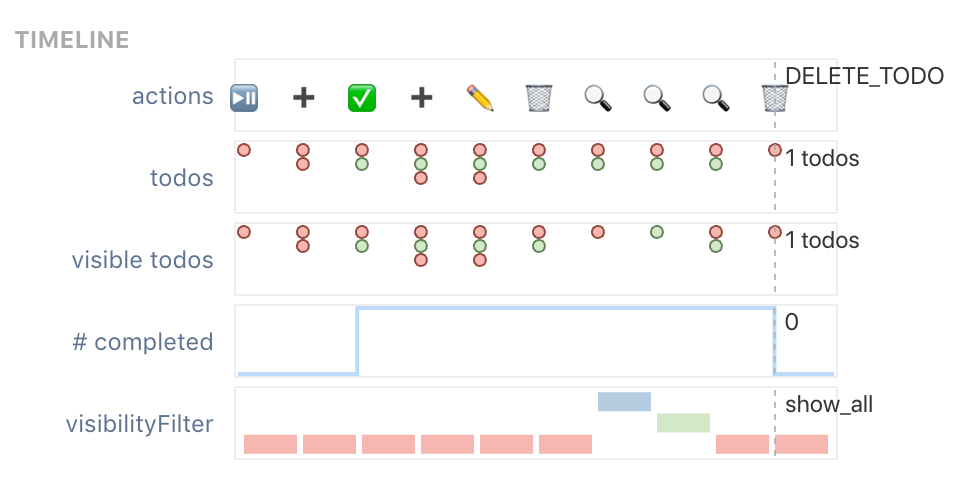
\includegraphics[width=3.4375in,height=2.08333in]{images/timeline.png}
\caption{Timeline view of stacked visualizations}\label{fig:timeline}
}
\end{figure}

One thing lost in the timeline view is the concrete view of the app's
entire state. It's still useful to see this, so I added a separate panel
which displays that data. The user can scrub through history in the
timeline, ``pin'' the app at a particular point in time, and then use
the separate state view to drill into the app's concrete state at that
point.

\hypertarget{visualization-types}{%
\subsection{Visualization Types}\label{visualization-types}}

Here are the specific types of visualizations I prototyped (all shown in
Figure~\ref{fig:timeline}):

\emph{Action list}: I found that skimming a list of actions represented
as text (``ADD\_TODO'', ``EDIT\_TODO'') required a lot of conscious
reading effort. Instead, by choosing a colorful symbol for each action
in the app, we can take advantage of pre-attentive processing to more
quickly understand what actions have occurred in the execution trace. In
this case I chose symbols for all the actions in TodoMVC; more
generally, a programmer could specify a meaningful symbol for every
action in their application. In some cases it might be difficult to
choose meaningful and different symbols for all actions; falling back to
random symbols or colored dots could work as well. In using this tool
I've found that the symbolic action list makes it far easier to find a
point in an execution trace that I'm looking for.

\emph{Line graph}: This is simply a line graph of some numeric quantity
over time. In this context I've used it to visualize quantities like
``Number of todos visible''. Choosing a y-axis is quite tricky because
the full range of values can't be known in advance. In trying out
different options and using the tool myself, I decided that viewing
relative changes over time was most important---generally I'm looking
for things like ``when did the number of todos go down?''. Therefore, I
let each graph scale to the current range of values and don't even show
a y-axis label---I'm not aiming to precisely read numeric values off the
graph.

\emph{Enum graph}: User interfaces commonly have enums / union types,
which can take on a small number of predefined values. To represent enum
values changing over time, I chose to use both a color and position
encoding, as a way of redundantly encoding the information and .

With more time, I'd like to explore many other types of visualizations
in addition to these. One particular interest is displaying the entire
state of a collection of objects in a single graph.

\hypertarget{prototype-implementation}{%
\subsection{Prototype Implementation}\label{prototype-implementation}}

I implemented a working prototype version of this visualization system.
I built a plugin on top of the existing Redux Dev Tools, which provides
substantial infrastructure for inspecting and manipulating the state of
a Redux application.

I used the React and Redux frameworks to implement the main skeleton of
my system. The graphs are built in a combination of d3 and React---using
d3 for computing scales and positions, and React for SVG rendering.

\hypertarget{sec:discussion}{%
\subsection{Discussion and Future Work}\label{sec:discussion}}

This work is still an early prototype and there are many opportunities
for future work.

Using this system myself, I found that I was able to more quickly get an
overall sense of what happened in an execution trace by looking at these
visualizations than looking at the existing Redux Dev Tools display.
However, I want to gain a clearer understanding of what questions people
have when learning about the behavior of a UI, in order to evaluate the
usefulness of the system. In particular, I'm curious about general
``program understanding'' as opposed to targeted debugging. Could this
visualization be a useful aid when onboarding someone into a codebase
and teaching them how it works?

There's lots of future work to refine the core visualizations further. I
haven't yet explored visualizing a complex object in a single graph, or
showing strings changing over time. I'd also like to more clearly
incorporate Hoffswell et al's taxonomy \autocite{hoffswell2018a} into
this work, evaluating these visualizations in those terms and explicitly
extending that taxonomy.

Another area of work is generalizing this system to work with any Redux
application. I'd like to explore the programmer experience of creating
these visualizations for an existing complex application. How much of
that process can be automated? How can we make it easy for the
programmer to decide which visualizations would be helpful, and then to
actually specify those visualizations? As an initial idea, I imagine
that the programmer could specify an arbitrary expression over the Redux
state,choose from a predefined list of visualizations for showing the
output of that expression, and then add that to the timeline panel in
this tool.

Program visualization offers a rich set of possibilities for helping
people understand their code better. In this work, I've provided an
initial prototype of a system for visualizing the runtime state of
Model-View-Update user interfaces, exploiting the natural architecture
of these applications to show an abstract picture of code execution over
time.

% Balancing columns in a ref list is a bit of a pain because you
% either use a hack like flushend or balance, or manually insert
% a column break.  http://www.tex.ac.uk/cgi-bin/texfaq2html?label=balance
% multicols doesn't work because we're already in two-column mode,
% and flushend isn't awesome, so I choose balance.  See this
% for more info: http://cs.brown.edu/system/software/latex/doc/balance.pdf
%
% Note that in a perfect world balance wants to be in the first
% column of the last page.
%
% If balance doesn't work for you, you can remove that and
% hard-code a column break into the bbl file right before you
% submit:
%
% http://stackoverflow.com/questions/2149854/how-to-manually-equalize-columns-
% in-an-ieee-paper-if-using-bibtex
%
% Or, just remove \balance and give up on balancing the last page.
%
\balance{}

% \bibliographystyle{SIGCHI-Reference-Format}
% \bibliography{sample}

\printbibliography

\end{document}

%%% Local Variables:
%%% mode: latex
%%% TeX-master: t
%%% End:
